\section{Flyweight}

O padrão Flyweight permite economizar o espaço em memória 
da aplicação ao fornecer uma instância compartilhada de 
uma classe para que ela não precise ser instanciada 
mais de uma vez. A figura \ref{flyweight_struct} mostra 
a estrutura do padrão. Nela, uma interface Flyweight 
define um elemento reutilizável, sendo implementada 
pelas classes ConcreteFlyweight e UnsharedConcreteFlyweight. 
A classe ConcreteFlyweight armazena um estado intrínseco 
e define uma operação que depende de um estado extrínseco 
para ser executada. 

Duas classes merecem atenção nesse diagrama. A primeira 
é a FlyweightFactory. Essa classe é adicionada para 
gerenciar a criação dos Flyweights e garantir que as 
instâncias da classe serão reutilizadas. Ela armazena, em 
seus atributos, uma lista de objetos Flyweight para que, 
quando o cliente solicitar, seja verificado se a instância 
desejada já existe. Caso não exista, ela é criada e 
adicionada à lista. 

A segunda classe que merece atenção é a UnsharedConcreteFlyweight, 
que é necessária caso existam elementos específicos 
do tipo Flyweight que não possam ser compartilhados. 
Esses elementos não podem ser criados através da 
FlyweightFactory.

\begin{figure}[htb]
	\caption{\label{flyweight_struct}Estrutura do Flyweight}
	\begin{center}
	    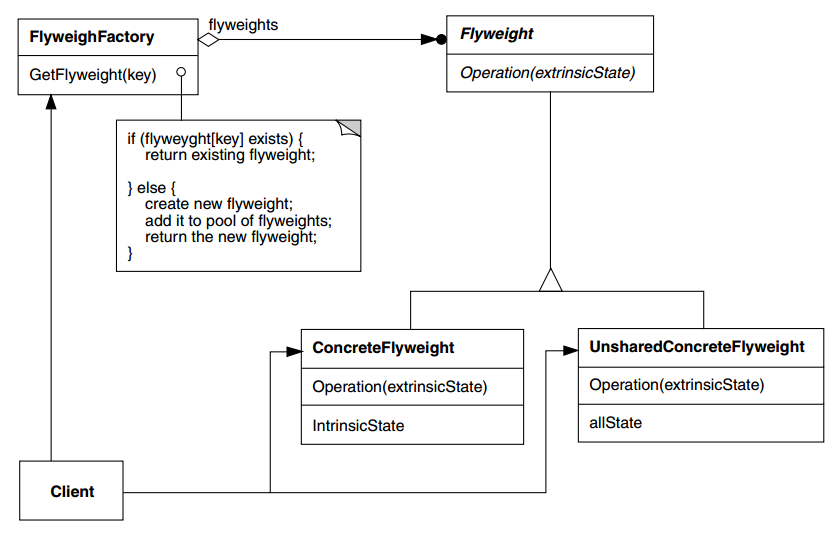
\includegraphics[scale=0.5]{5_padroes-contexto-funcional/5.2_estruturais/5.2.6_flyweight/diagram.png}
	\end{center}
\end{figure}

\subsection*{Exemplo Orientado a Objetos}

Um editor de documentos possui uma ferramenta 
de formatação e edição de textos. Para reduzir o 
custo de memória, as classes que armazenam os 
caracteres do alfabeto devem ser compartilhadas, 
dada a quantidade de instâncias de um mesmo caracter 
que existiriam em um texto com centenas de palavras. 
Ao mesmo tempo, a ferramenta deve armazenar dois 
elementos que não podem ser compartilhados com as 
letras - a linha e a coluna onde cada letra está 
localizada. 

A figura \ref{flyweight_exemplo} apresenta o diagrama 
de classes para esse exemplo. A interface Glyph 
representa um elemento textual. As classes Row e 
Column armazenam em seus atributos um conjunto de objetos 
do tipo Glyph. 
Por fim, a classe Character armazena em seus atributos 
o caracter que deve ser compartilhado. Apenas uma 
instância é criada para cada caracter. O 
código \ref{ooflyweight} demonstra a implementação 
desse exemplo.

\begin{figure}[htb]
	\caption{\label{flyweight_exemplo}Exemplo de Flyweight}
	\begin{center}
	    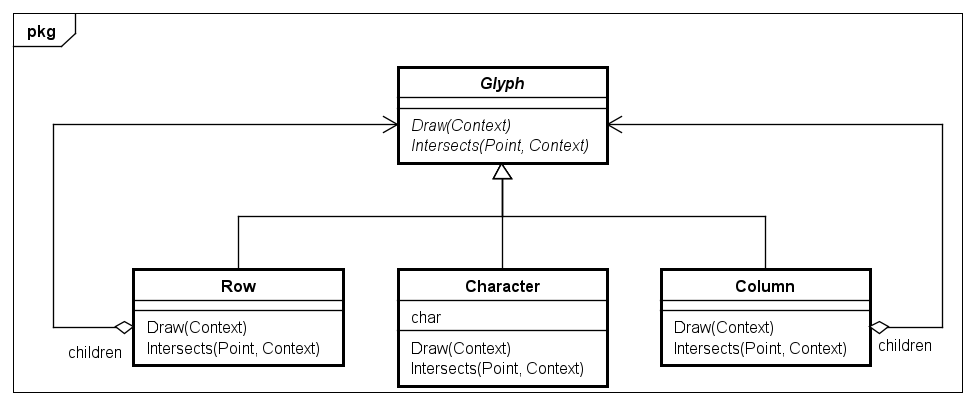
\includegraphics[scale=0.45]{5_padroes-contexto-funcional/5.2_estruturais/5.2.6_flyweight/flyweight_exemplo.png}
	\end{center}
\end{figure}

\begin{lstlisting}[caption={Flyweight Orientado a Objetos},label=ooflyweight]

trait Glyph {
	def Draw(context : Context);
	def Intersects(point : Point, context : Context);
}

class Character(val c) extends Glyph {
	def Draw(context : Context) {
		// Desenha o caracter
	}

	def Intersects(point : Point, context : Context) {
		// Verifica a interseção com o ponto
	}
}

class Row(var children : List[Glyph]) extends Glyph {

	def Draw(context : Context) {
		// Desenha a linha
	}

	def Intersects(point : Point, context : Context) {
		// Verifica a interseção com o ponto
	}
}

class Column(var children : List[Glyph]) extends Glyph {

	def Draw(context : Context) {
		// Desenha a coluna
	}

	def Intersects(point : Point, context : Context) {
		// Verifica a interseção com o ponto
	}
}


\end{lstlisting}

\subsection*{Contexto Funcional}

\begin{comment}
A ideia do Flyweight assemelha-se à de memoização, onde o 
retorno de uma função pura é armazenado para que seu valor 
não precise ser recalculado quando os mesmos parâmetros 
são passados. Essa abordagem só é possível para funções 
puras pois, caso ocorram efeitos colaterais ou a função 
dependa de dados externos, o resultado pode ser diferente 
para os mesmos parâmetros, gerando um resultado não 
confiável.

Apesar da ideia de memoização parecer mais focada no tempo 
de execução no que no espaço em memória, dependendo da 
implementação é possível economizar ambos.
\end{comment}

\begin{lstlisting}[caption={Flyweight Funcional},label=fpflyweight]
    

    
\end{lstlisting}